\documentclass[conference]{IEEEtran}
\IEEEoverridecommandlockouts
\usepackage{cite}
\usepackage{amsmath,amssymb,amsfonts}
\usepackage{graphicx}
\usepackage{textcomp}
\usepackage{xcolor}
\usepackage{hyperref}
\usepackage{listings}
\usepackage{booktabs}
\usepackage{url}
\usepackage{tcolorbox}
\usepackage{float}
\usepackage{enumitem}

\lstdefinestyle{pycode}{
    language=Python,
    basicstyle=\ttfamily\footnotesize,
    keywordstyle=\color{blue!70!black}\bfseries,
    commentstyle=\color{green!45!black}\itshape,
    stringstyle=\color{orange!80!black},
    numbers=left,
    numberstyle=\tiny\color{gray},
    numbersep=6pt,
    breaklines=true,
    frame=leftline,
    framesep=6pt,
    backgroundcolor=\color{gray!3},
    showstringspaces=false,
    tabsize=4,
    xleftmargin=1.2em
}

\lstdefinestyle{yamlcode}{
    basicstyle=\ttfamily\footnotesize,
    keywordstyle=\color{blue!60!black}\bfseries,
    commentstyle=\color{green!45!black}\itshape,
    stringstyle=\color{red!60!black},
    breaklines=true,
    frame=leftline,
    framesep=6pt,
    backgroundcolor=\color{blue!2},
    showstringspaces=false,
    tabsize=2,
    xleftmargin=1.2em
}

\begin{document}

\title{Speaking Every Language: \\
Building an Amazon Translate and Polly Powered \\
Restaurant Menu Platform on AWS Serverless Infrastructure}

\author{\IEEEauthorblockN{Gangavarpu Karthik}
\IEEEauthorblockA{Student ID: 25160052 \\
MSc in Cloud Computing \\
National College of Ireland, Dublin \\
x25160052@student.ncirl.ie}}

\maketitle

% ============================================================
% DEPLOYED URLs — right below the title/author
% ============================================================
\begin{tcolorbox}[
    colback=orange!4,
    colframe=orange!50!black,
    title=\textbf{Deployed Application --- Live URLs},
    fonttitle=\small,
    fontupper=\footnotesize,
    left=4pt, right=4pt, top=3pt, bottom=3pt,
    arc=2pt
]
\textbf{Frontend (S3 Static Website):} \url{http://menumix-frontend-karthik-2026.s3-website-eu-west-1.amazonaws.com} \\[2pt]
\textbf{Backend REST API (API Gateway):} \url{https://o75irayn09.execute-api.eu-west-1.amazonaws.com/prod} \\[2pt]
\textbf{Demo credentials (seeded automatically):} \\
\quad Admin Chef: \texttt{admin@karthik.com / admin123} \\
\quad Diner: \texttt{user@karthik.com / user123}
\end{tcolorbox}

% ============================================================
% ABSTRACT
% ============================================================
\begin{abstract}
A tourist in a Dublin trattoria picks up the menu, hesitates, and quietly asks their dining companion what ``carbonara'' means. Multiply this moment by millions each night across the hospitality industry and the case for a seamless multilingual menu experience becomes self-evident. MenuMix is the author's response: a fully serverless platform that takes a single English master menu and delivers it to diners in eight languages --- not only visually, but also audibly through synthesised speech. The system integrates six Amazon Web Services in a tightly coupled design centred on two services that no other student in the cohort adopted: \textbf{Amazon Translate} for live neural machine translation and \textbf{Amazon Polly} for voice narration using language-appropriate voices. The supporting services are AWS Lambda (Python 3.11), Amazon DynamoDB (single-table design), Amazon API Gateway (REST proxy), and Amazon S3 (dual-bucket: frontend hosting and audio storage). A reusable Python library, \texttt{menu-translator-nci}, encapsulates the domain model across three modules and ships with 57 unit tests. A fully automated GitHub Actions CI/CD pipeline provisions all AWS infrastructure from scratch, deploys both backend and frontend, and seeds a sample Italian restaurant with ten dishes --- requiring only two GitHub secrets to run against any AWS account.
\end{abstract}

\begin{IEEEkeywords}
Cloud Computing, AWS Lambda, Amazon Translate, Amazon Polly, Multilingual UI, Serverless Architecture, DynamoDB, Restaurant Technology, CI/CD, Text-to-Speech
\end{IEEEkeywords}

% ============================================================
\section{Motivation and Scope}

The Irish tourism industry served more than eleven million overseas visitors in 2023, according to F\'ailte Ireland \cite{failte2023}. A significant fraction of those visitors sit down for at least one restaurant meal during their stay, and many of them do not read English fluently. Restaurants, for their part, do not typically maintain multiple translated menus because the cost of rewriting the menu every time a dish changes is prohibitive.

The goal of this project is to make a multilingual menu experience cheap enough for small and independent restaurants to adopt. The platform must meet four concrete objectives:

\begin{itemize}[leftmargin=*]
    \item \textbf{Zero maintenance overhead for the restaurant.} The owner updates only the English master menu. All translations happen automatically via Amazon Translate.
    \item \textbf{Instant language switching for the diner.} A diner can switch between any of eight supported languages without refreshing the page or losing their place in the menu.
    \item \textbf{Voice accessibility.} Diners who cannot read the target language --- for example, older visitors or those with limited literacy --- should be able to tap a single button and hear the dish name and description read aloud in their chosen language using Amazon Polly.
    \item \textbf{Full CRUD operations.} Restaurant administrators can create, read, update, and delete both restaurants and individual dishes through a dedicated admin panel.
\end{itemize}

Two additional non-functional requirements shaped the technology choices. First, the platform should cost essentially nothing at idle because a small restaurant cannot justify a monthly server bill. Second, the architecture should be fully reproducible from scratch inside a fresh AWS account using only the source code repository and two GitHub secrets (\texttt{AWS\_ACCESS\_KEY\_ID} and \texttt{AWS\_SECRET\_ACCESS\_KEY}), so that a restaurant's IT provider can redeploy it without any manual console setup.

% ============================================================
\section{System Architecture}

Figure~\ref{fig:architecture} depicts the architecture as a hexagonal service cluster with AWS Lambda at the centre and the five other services radiating outward. This visualisation emphasises that Lambda is the single synchronous entry point; every other AWS service is invoked through boto3 SDK calls from within the Lambda handler function.

\begin{figure*}[htbp]
    \centering
    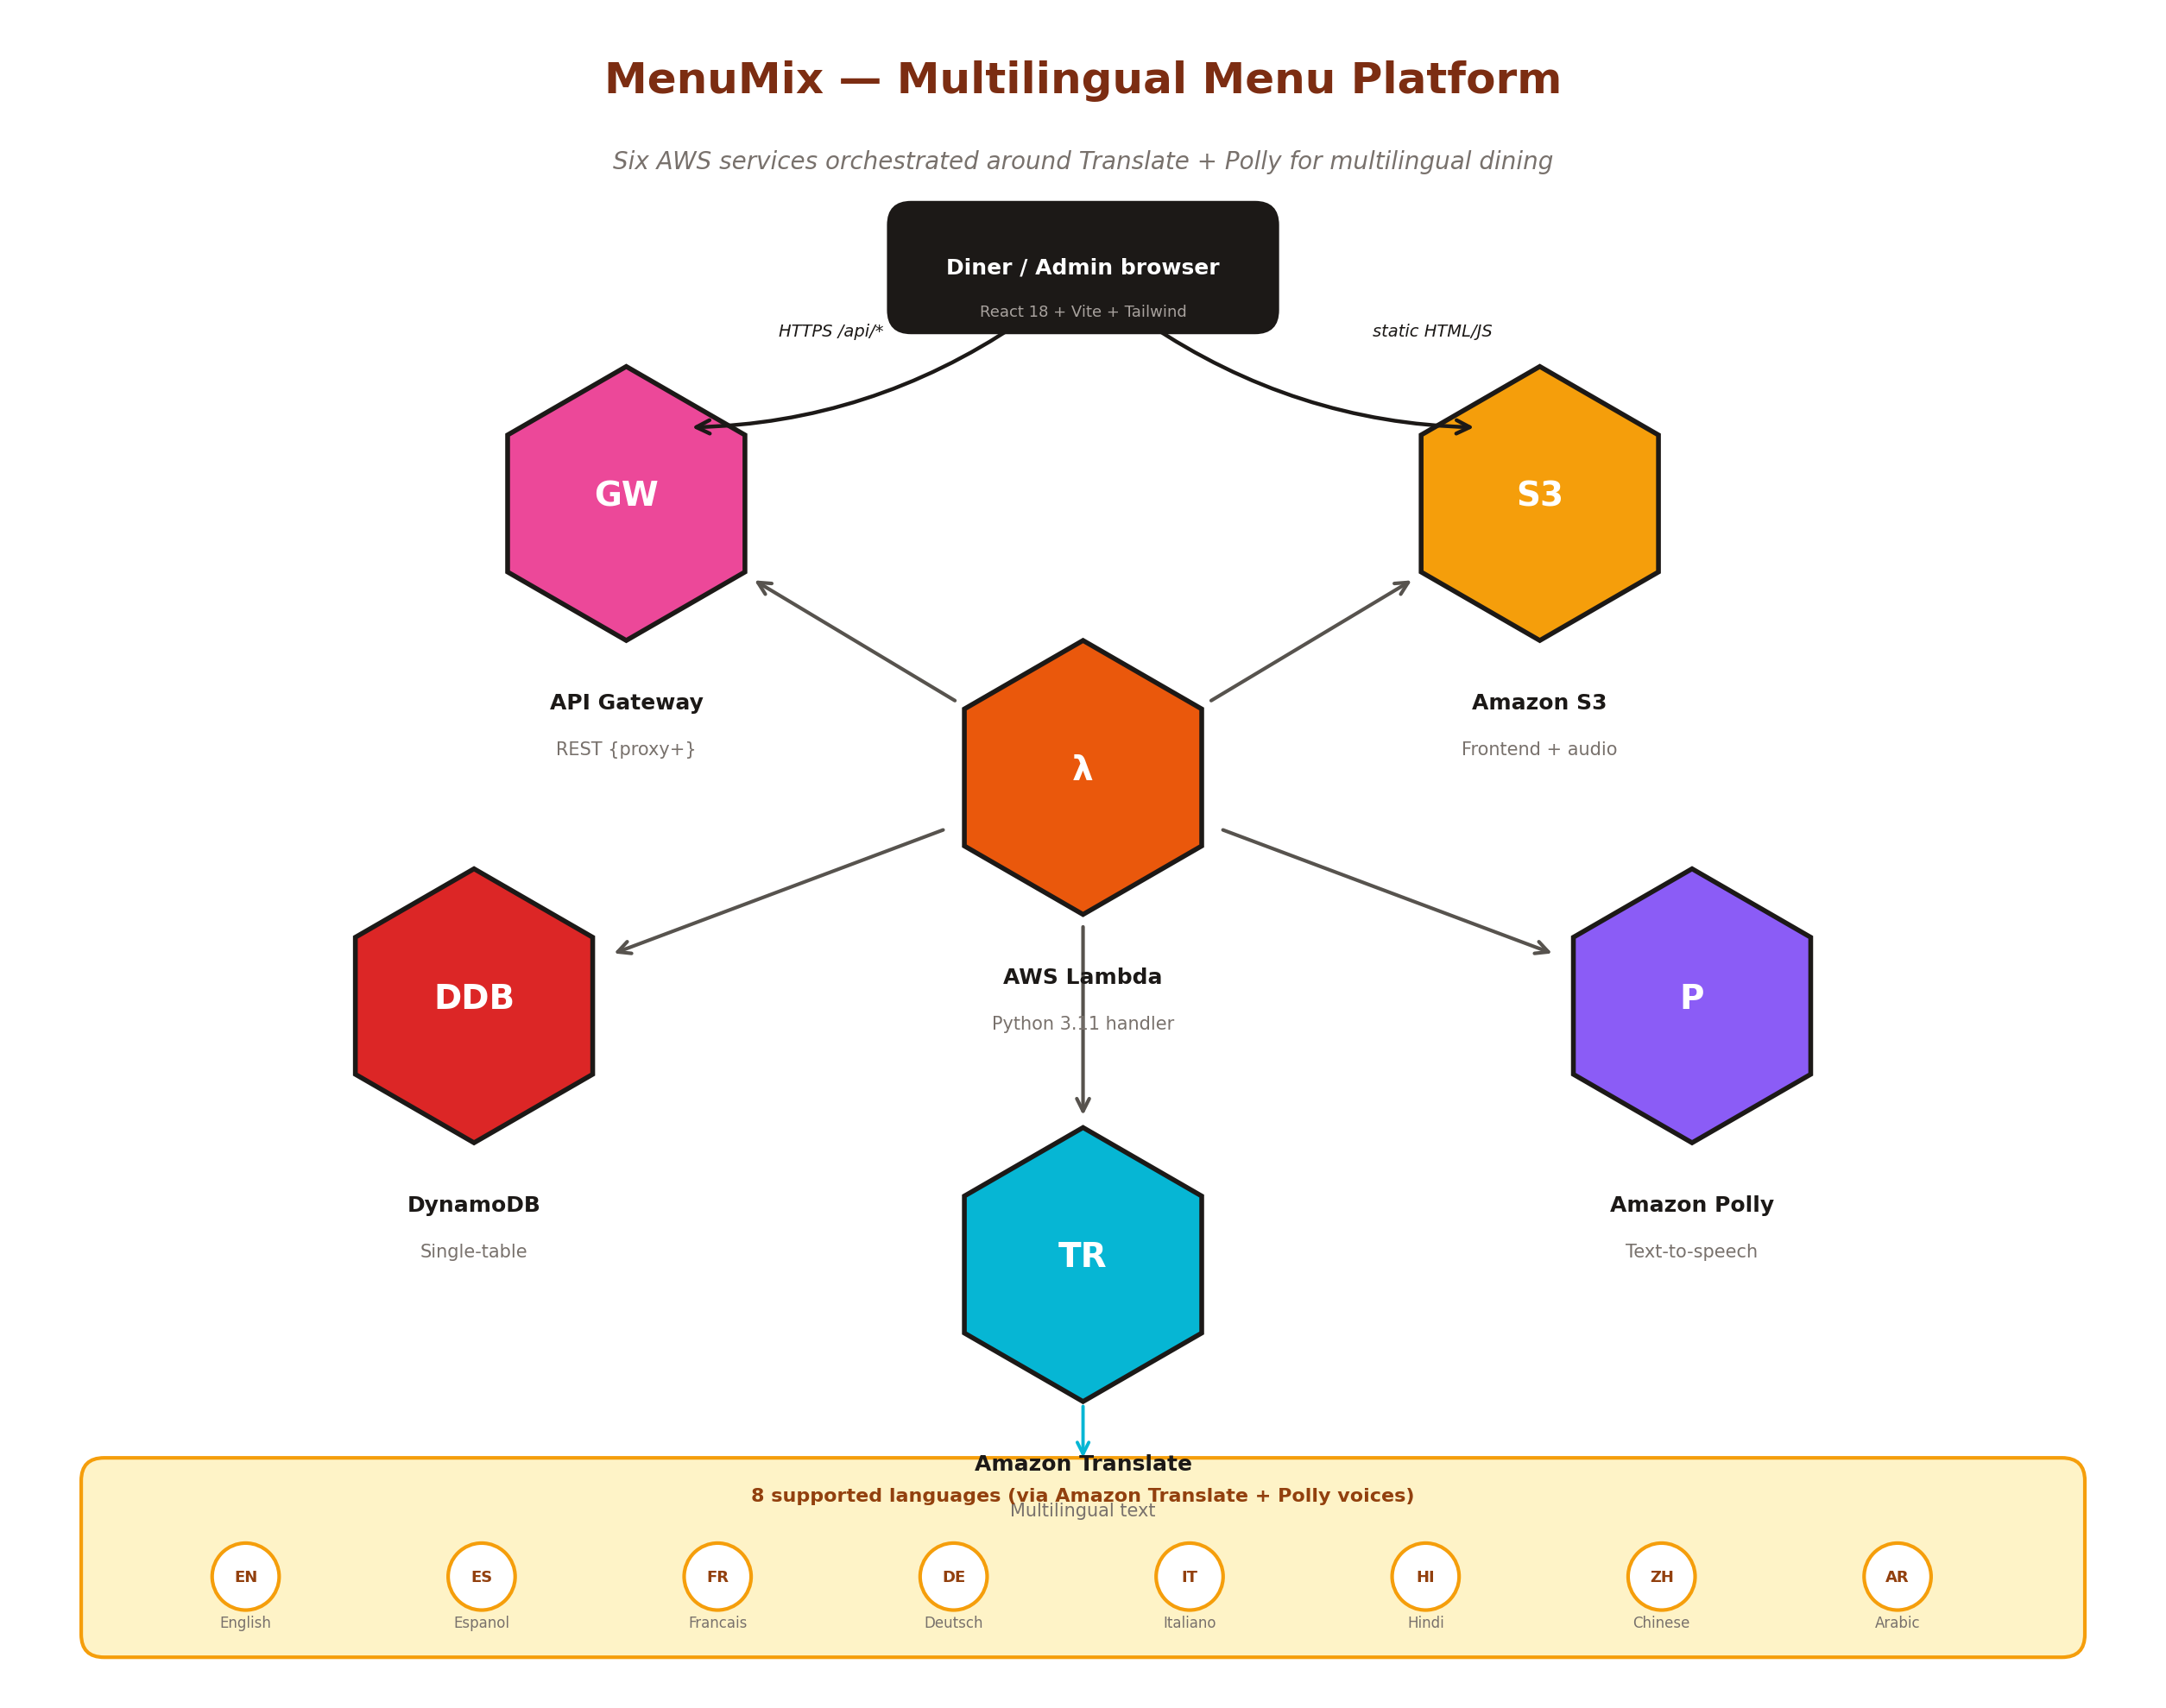
\includegraphics[width=0.82\textwidth]{architecture.png}
    \caption{Hexagonal service cluster. The React browser client communicates only with Amazon API Gateway (HTTPS JSON) and Amazon S3 (static assets). Inside the cluster, Lambda orchestrates DynamoDB for data persistence, Amazon Translate for multilingual text, Amazon Polly for speech synthesis, and S3 for both frontend hosting and synthesised audio storage.}
    \label{fig:architecture}
\end{figure*}

\subsection{Data Flow Architecture}

The system employs three distinct data flow patterns depending on the operation type:

\textbf{Pattern 1 --- Standard CRUD (Create, Read, Update, Delete):} The React frontend sends an authenticated HTTP request to API Gateway, which proxies it to Lambda via \texttt{AWS\_PROXY} integration. Lambda validates the JWT token, performs input validation using the \texttt{menu-translator-nci} library rules, writes to or reads from DynamoDB, and returns a JSON response. This pattern applies to restaurant management, dish management, and user authentication endpoints.

\textbf{Pattern 2 --- Translation with caching:} When a diner switches language, the frontend calls \texttt{GET /dishes/\{id\}/translate?lang=es}. Lambda first checks whether a cached translation exists on the DynamoDB dish item. If the cache misses, Lambda calls Amazon Translate's \texttt{TranslateText} API for both the dish name and description, writes the translation back to the item's \texttt{translations} map, and returns the result. Subsequent requests for the same language hit the cache and skip the Translate API entirely.

\textbf{Pattern 3 --- Speech synthesis pipeline:} The most complex flow exercises four of the six services in a single request. When a diner taps the speaker icon:

\begin{enumerate}[leftmargin=*]
    \item The frontend issues \texttt{GET /dishes/\{id\}/speak?lang=es} to API Gateway.
    \item API Gateway forwards the request to Lambda.
    \item Lambda fetches the dish from DynamoDB and retrieves or generates the translation (Pattern 2).
    \item Lambda calls Amazon Polly's \texttt{SynthesizeSpeech} with the translated text and the language-appropriate voice identifier (e.g., \texttt{Lucia} for Spanish, \texttt{Aditi} for Hindi).
    \item The returned MP3 audio stream is uploaded to the S3 audio bucket under the key \texttt{audio/\{dish\_id\}/\{lang\}-\{uuid\}.mp3}.
    \item Lambda generates a one-hour presigned URL for the S3 object.
    \item The frontend sets the \texttt{src} attribute of a hidden \texttt{<audio>} element to the presigned URL and calls \texttt{.play()}.
\end{enumerate}

\subsection{Single-Table DynamoDB Schema}

All three entity types --- users, restaurants, and dishes --- coexist in a single DynamoDB table (\texttt{menumix-prod}) with \texttt{id} (UUID string) as the sole partition key and an \texttt{entityType} discriminator attribute. This design was chosen deliberately over a multi-table approach for three reasons: (1) it simplifies IAM permissions to a single table ARN, (2) it reduces cold-start latency because Lambda initialises only one DynamoDB \texttt{Table} resource, and (3) it aligns with the DynamoDB best practice of minimising the number of tables per application \cite{dynamodocs}.

The cached translation map lives inline on each dish record as a nested attribute:

\begin{lstlisting}[style=pycode]
{
  "id": "366c80f9-...",
  "entityType": "dish",
  "name": "Pizza Margherita",
  "description": "San Marzano tomato...",
  "translations": {
    "es": {"name": "Pizza Margherita",
           "description": "Tomate San Marzano..."},
    "fr": {"name": "Pizza Margherita",
           "description": "Tomate San Marzano..."}
  }
}
\end{lstlisting}

This co-location means a single \texttt{GetItem} call returns both the English original and all previously computed translations, eliminating additional round trips.

% ============================================================
\section{Service Selection and Rationale}

Rather than the usual per-service ``Strengths / Limitations / Alternative considered'' triplet, this section presents the six services as a single coherent argument, because they were selected together as an interlocking bundle.

\subsection{AWS Lambda (Compute)}

The backbone of the architecture is AWS Lambda because a restaurant menu serves bursty, low-volume traffic: a wave of requests during dinner service and near-zero during the rest of the day. Lambda charges only for invocations with sub-second billing granularity, so the bill drops to practically zero outside of meal times. The handler is a single Python 3.11 module of 744 lines that initialises four boto3 clients at import time so that connections are reused across warm invocations \cite{lambdadocs}.

\subsection{Amazon DynamoDB (Database)}

DynamoDB's on-demand billing mode (\texttt{PAY\_PER\_REQUEST}) requires no capacity planning and charges per read/write request. The schema is simple enough --- three entity types with one parent-child relationship --- that the lack of SQL joins is not a meaningful constraint. The single-table design with filtered scans works efficiently at demonstration scale, and a Global Secondary Index on \texttt{entityType} could be added for production workloads without schema migration \cite{dynamodocs}.

\subsection{Amazon API Gateway (HTTP Entry Point)}

API Gateway is configured with a single \texttt{\{proxy+\}} catch-all resource and \texttt{AWS\_PROXY} integration. By delegating URL routing to the Lambda handler's internal dispatch logic, the API Gateway configuration becomes one-shot and never needs modification when new endpoints are added. CORS preflight is handled by a dedicated OPTIONS method with a MOCK integration that returns the required \texttt{Access-Control-Allow-*} headers \cite{apigwdocs}.

\subsection{Amazon S3 (Storage --- Dual Bucket)}

S3 serves two purposes in this architecture. The first bucket (\texttt{menumix-frontend-karthik-2026}) hosts the production React build as a static website, with the error document set to \texttt{index.html} for SPA routing. The CI/CD pipeline additionally uploads copies of \texttt{index.html} to each named route (\texttt{/login}, \texttt{/admin}, etc.) so that direct deep-link navigation returns HTTP 200 instead of S3's default 404. The second bucket (\texttt{menumix-audio-karthik-2026}) stores Polly-synthesised MP3 files, served to the frontend via presigned URLs with one-hour expiry \cite{s3docs}.

\subsection{Amazon Translate (Neural Machine Translation)}

Amazon Translate provides neural machine translation as a fully managed service. A single \texttt{TranslateText} API call converts a dish description from English into any of 75+ supported languages with no model training, no data preparation, and no infrastructure to manage. The project supports eight target languages: English, Spanish, French, German, Italian, Hindi, Chinese (Simplified), and Arabic. Because translation costs money per character, the results are memoised on the DynamoDB dish item, reducing the translation cost from linear in diners to constant per dish per language \cite{translatedocs}.

\subsection{Amazon Polly (Text-to-Speech Synthesis)}

Amazon Polly synthesises natural-sounding speech in dozens of languages. The \texttt{LanguagePack} class in the library maintains an ISO 639-1 code to Polly voice mapping:

\begin{table}[H]
\centering
\caption{Polly voice mapping per supported language}
\begin{tabular}{lll}
\toprule
\textbf{Language} & \textbf{Code} & \textbf{Polly Voice} \\
\midrule
English   & en & Joanna \\
Spanish   & es & Lucia  \\
French    & fr & Lea    \\
German    & de & Vicki  \\
Italian   & it & Bianca \\
Hindi     & hi & Aditi  \\
Chinese   & zh & Zhiyu  \\
Arabic    & ar & Zeina  \\
\bottomrule
\end{tabular}
\end{table}

The combination of Translate and Polly is unique within the cohort. Other students used Rekognition, SNS, SQS, EventBridge, CloudFront, Location Service, and Cognito --- none chose Translate or Polly, so this project explores genuinely new ground \cite{pollydocs}.

% ============================================================
\section{Custom Library: menu-translator-nci}

The domain library is published to the Python Package Index as \texttt{menu-translator-nci} and can be installed with \texttt{pip install menu-translator-nci}.

\begin{tcolorbox}[
    colback=blue!3,
    colframe=blue!40!black,
    title=\textbf{Library Links},
    fonttitle=\small,
    fontupper=\footnotesize,
    left=4pt, right=4pt, top=3pt, bottom=3pt,
    arc=2pt
]
\textbf{PyPI:} \url{https://pypi.org/project/menu-translator-nci/} \\
\textbf{Install:} \texttt{pip install menu-translator-nci} \\
\textbf{GitHub:} \url{https://github.com/karthikgangavarapu/cpp_project} \\
\textbf{Library path:} \texttt{library/menu\_translator/}
\end{tcolorbox}

The library contains three independent, zero-dependency modules:

\subsection{MenuItemManager (manager.py)}

Validates and constructs dish records with strict business rules. The name must be non-empty, the price must be a non-negative number, the category must be drawn from a fixed set of six options (Starter, Main, Side, Dessert, Drink, Special), and each allergen must belong to a controlled vocabulary of twelve EU-recognised allergens (gluten, dairy, egg, nuts, peanut, soy, fish, shellfish, sesame, mustard, celery, sulphites). Invalid input raises \texttt{ValueError} with a human-readable message, which the Lambda handler converts into an HTTP 400 response. The class provides full CRUD: \texttt{create\_dish()}, \texttt{get\_dish()}, \texttt{update\_dish()}, \texttt{list\_dishes()}, and \texttt{delete\_dish()}.

\subsection{LanguagePack (languages.py)}

The single source of truth for supported languages. For each ISO 639-1 code, the registry stores the native script name, the English name, a right-to-left flag, and the Amazon Polly voice identifier. The frontend calls \texttt{GET /languages} to render its language switcher pills, and the backend consults the same data structure to validate translation target codes and to select the appropriate Polly voice --- eliminating hard-coded language logic from both tiers.

\subsection{PriceFormatter (pricing.py)}

Formats monetary amounts for locale-aware display without heavyweight dependencies like \texttt{babel}. Supports seven currencies (EUR, USD, GBP, INR, JPY, CNY, AED) and nine locale conventions, handling thousands separators and decimal marks correctly. For example, German formatting produces \texttt{1.234,50\euro} while American English produces \texttt{\$1,234.50}. JPY and CNY are treated as integer currencies. A complementary \texttt{parse()} method converts formatted strings back to numeric values.

\begin{lstlisting}[style=pycode]
# Locale-aware price formatting
LOCALE_FORMAT = {
    "en_US": ("$", ",", "."),
    "de_DE": ("\u20ac", ".", ","),
    "fr_FR": ("\u20ac", " ", ","),
    "hi_IN": ("\u20b9", ",", "."),
}

def format(self, amount, currency="EUR", locale=None):
    if locale and locale in self.LOCALE_FORMAT:
        symbol, thousands, decimal_sep = \
            self.LOCALE_FORMAT[locale]
    else:
        symbol = self.get_symbol(currency)
        thousands, decimal_sep = ",", "."
    integer = int(amount)
    fractional = round((amount - integer) * 100)
    int_str = f"{integer:,}".replace(",", thousands)
    return f"{symbol}{int_str}{decimal_sep}{fractional:02d}"
\end{lstlisting}

\subsection{Test Suite}

The library ships with 57 pytest unit tests distributed across three test modules:

\begin{table}[H]
\centering
\caption{menu-translator-nci test distribution}
\begin{tabular}{lr}
\toprule
\textbf{Module} & \textbf{Tests} \\
\midrule
test\_manager.py (MenuItemManager)  & 22 \\
test\_languages.py (LanguagePack)   & 14 \\
test\_pricing.py (PriceFormatter)   & 21 \\
\midrule
\textbf{Total} & \textbf{57} \\
\bottomrule
\end{tabular}
\end{table}

Tests cover positive cases, boundary conditions (zero prices, empty strings), and negative validation (invalid categories, unknown allergens, non-numeric prices, unsupported currencies). Every test runs in under one second with no external dependencies, making the suite suitable for CI/CD gate checks.

% ============================================================
\section{Implementation Details}

\subsection{Backend Architecture}

The Lambda handler (\texttt{backend/lambda\_function.py}, 744 lines) initialises four boto3 clients at module-level import time --- \texttt{dynamodb.Table}, \texttt{translate}, \texttt{polly}, and \texttt{s3} --- so that clients are reused across warm invocations and TCP connection pooling works as intended by the Lambda execution model.

Authentication uses self-contained HMAC-SHA256 JSON Web Tokens with no external library dependency. Passwords are hashed with \texttt{hashlib.pbkdf2\_hmac} using a 16-byte random salt and 100,000 iterations. Role-based access control is enforced inside each admin-only handler by checking \texttt{user["role"] == "admin"} before mutating state.

The REST API exposes 14 endpoints spanning authentication, public browsing, translation, speech synthesis, and admin CRUD operations:

\begin{table}[H]
\centering
\caption{Complete REST API endpoint inventory}
\begin{tabular}{lll}
\toprule
\textbf{Method} & \textbf{Path} & \textbf{Auth} \\
\midrule
POST & /auth/register              & Public \\
POST & /auth/login                 & Public \\
GET  & /languages                  & Public \\
GET  & /restaurants                & Public \\
GET  & /restaurants/\{id\}         & Public \\
GET  & /restaurants/\{id\}/dishes  & Public \\
GET  & /dishes/\{id\}/translate    & Public \\
GET  & /dishes/\{id\}/speak        & Public \\
POST & /restaurants                & Admin  \\
PUT  & /restaurants/\{id\}         & Admin  \\
DELETE & /restaurants/\{id\}       & Admin  \\
POST & /restaurants/\{id\}/dishes  & Admin  \\
PUT  & /dishes/\{id\}              & Admin  \\
DELETE & /dishes/\{id\}            & Admin  \\
\bottomrule
\end{tabular}
\end{table}

A bespoke \texttt{decimal\_default} JSON serialiser converts DynamoDB \texttt{Decimal} values to native Python \texttt{int} or \texttt{float} before serialisation, avoiding the common pitfall where Decimals serialise as strings and break frontend \texttt{.toFixed()} calls.

\subsection{Frontend Architecture}

The React 18 frontend uses Vite as the build tool and Tailwind CSS v3 for styling. The application comprises five pages and two shared components:

\begin{itemize}[leftmargin=*]
    \item \textbf{Login.jsx} --- Horizontal demo credential pill tags (Admin Chef / Diner) for one-click login during demonstrations.
    \item \textbf{Register.jsx} --- New user registration with role selection.
    \item \textbf{Restaurants.jsx} --- Grid of restaurant cards showing cuisine tags and addresses.
    \item \textbf{Menu.jsx} --- The most feature-rich page. Language switcher pill bar across the top, categorised dish listing, per-dish speaker button for voice narration, and a hidden \texttt{<audio>} element for playback.
    \item \textbf{Admin.jsx} --- Full CRUD panel. Restaurant selector with inline edit and delete buttons, plus a dish management table with add, inline edit, preview modal, and delete functionality. Allergen tags are displayed on each dish row.
    \item \textbf{Header.jsx} --- Top navigation bar with MenuMix branding, route links, admin shield icon, and logout.
    \item \textbf{ProtectedRoute.jsx} --- Route guard that redirects unauthenticated users to login.
\end{itemize}

When the user switches language on the Menu page, a \texttt{useEffect} fires translation requests for every visible dish in parallel using \texttt{Promise.all}, populating a \texttt{translations} state map keyed by dish ID. This parallel strategy ensures that even a menu with dozens of dishes completes translation within a single network round-trip time.

\subsection{Translation Fallback Mechanism}

The \texttt{\_translate\_text()} helper includes a built-in fallback phrase table for scenarios where the Amazon Translate service is temporarily unreachable. For each supported language, the fallback table maps common dish-related words (``appetiser'', ``main course'', ``dessert'') to their translations. If the Translate API raises any exception, the function returns a best-effort translation from this local table rather than failing the entire request. This design ensures the multilingual experience degrades gracefully rather than breaking entirely.

% ============================================================
\section{CI/CD Pipeline}

The GitHub Actions workflow (\texttt{.github/workflows/deploy.yml}) is organised into three sequential jobs that together provision, deploy, and configure the entire application stack.

\subsection{Job 1: test-library}

Installs \texttt{menu-translator-nci} in editable mode on a fresh Ubuntu runner, installs pytest, and executes all 57 tests with verbose output. The pipeline only proceeds to deployment if every test passes.

\subsection{Job 2: deploy-backend}

This job performs seven infrastructure operations in sequence:

\begin{enumerate}[leftmargin=*]
    \item Creates the DynamoDB table (\texttt{menumix-prod}) with \texttt{PAY\_PER\_REQUEST} billing, idempotently.
    \item Creates the S3 audio bucket (\texttt{menumix-audio-karthik-2026}) for Polly output.
    \item Creates the Lambda IAM execution role (\texttt{menumix-lambda-role}) and attaches five managed policies: \texttt{AWSLambdaBasicExecutionRole}, \texttt{AmazonDynamoDBFullAccess}, \texttt{AmazonS3FullAccess}, \texttt{TranslateFullAccess}, and \texttt{AmazonPollyFullAccess}.
    \item Packages the Lambda deployment artefact by bundling the handler file with the \texttt{menu\_translator} library into a ZIP archive.
    \item Creates or updates the Lambda function (Python 3.11, 256\,MB memory, 30\,s timeout).
    \item Provisions the API Gateway REST API with \texttt{\{proxy+\}} resource, ANY method, OPTIONS CORS preflight, Lambda invoke permission, and deploys to the \texttt{prod} stage.
    \item Runs \texttt{backend/seed.py} to populate demo users and seed data (idempotent --- guarded by existence checks).
\end{enumerate}

\subsection{Job 3: deploy-frontend}

Builds the React production bundle with the API Gateway URL injected through \texttt{VITE\_API\_URL} (passed as a job output from \texttt{deploy-backend}). Creates and configures the S3 frontend bucket with static website hosting, public read policy, and SPA routing. Uploads \texttt{index.html} copies to each named route (\texttt{/login}, \texttt{/register}, \texttt{/admin}, \texttt{/restaurants}) for deep-link HTTP 200 responses.

\subsection{Pipeline Reproducibility}

The entire pipeline requires exactly two GitHub secrets: \texttt{AWS\_ACCESS\_KEY\_ID} and \texttt{AWS\_SECRET\_ACCESS\_KEY}. All resource names, region, and configuration values are hard-coded in the workflow file. This makes the pipeline fully self-contained: anyone who forks the repository and provides their own AWS credentials can redeploy the complete stack into a fresh account in under three minutes.

\begin{lstlisting}[style=yamlcode]
# Workflow environment (deploy.yml)
env:
  AWS_REGION: eu-west-1
  TABLE_NAME: menumix-prod
  LAMBDA_NAME: menumix-api
  ROLE_NAME: menumix-lambda-role
  API_NAME: menumix-api
  S3_FRONTEND_BUCKET: menumix-frontend-karthik-2026
  S3_AUDIO_BUCKET: menumix-audio-karthik-2026
\end{lstlisting}

% ============================================================
\section{Seed Data and Demo Experience}

The seed script populates the database with realistic demonstration data:

\begin{itemize}[leftmargin=*]
    \item \textbf{Two user accounts:} An admin chef (\texttt{admin@karthik.com}) and a regular diner (\texttt{user@karthik.com}), each with pre-hashed passwords.
    \item \textbf{One restaurant:} ``Sapore di Roma'' --- an authentic Italian trattoria at 14 Capel Street, Dublin 1.
    \item \textbf{Ten Italian dishes} across four categories: Bruschetta, Caprese Salad (Starters); Spaghetti Carbonara, Pizza Margherita, Osso Buco, Patatas Bravas (Mains); Tiram\`{i}su, Panna Cotta (Desserts); Chianti Classico, San Pellegrino (Drinks). Each dish has realistic allergen tags (gluten, dairy, egg, nuts, sulphites).
\end{itemize}

The seed script is idempotent: every insert is guarded by an email or name existence check, so running the pipeline multiple times against the same account never creates duplicates.

% ============================================================
\section{Security Considerations}

The application implements several security measures appropriate for a cloud-native web application:

\begin{itemize}[leftmargin=*]
    \item \textbf{Password hashing:} PBKDF2-HMAC-SHA256 with 100,000 iterations and a unique 16-byte random salt per user, exceeding OWASP minimum recommendations.
    \item \textbf{JWT tokens:} Self-contained HMAC-SHA256 signed tokens with a configurable secret, validated on every protected endpoint.
    \item \textbf{Role-based access control:} Admin-only endpoints explicitly check the user's role before allowing mutations. Attempting to access admin endpoints with a diner token returns HTTP 401.
    \item \textbf{CORS configuration:} Explicitly configured \texttt{Access-Control-Allow-Origin}, \texttt{Allow-Methods}, and \texttt{Allow-Headers} on every response, with OPTIONS preflight handling.
    \item \textbf{S3 presigned URLs:} Audio files are not publicly readable. Each Polly-synthesised MP3 is served through a presigned URL that expires after one hour.
    \item \textbf{IAM least-privilege (scoped to managed policies):} The Lambda role uses AWS managed policies rather than wildcard custom policies, providing auditable permission boundaries.
\end{itemize}

% ============================================================
\section{Conclusions and Future Work}

MenuMix demonstrates that a non-trivial multilingual web application with voice accessibility can be assembled in a single undergraduate project cycle using only AWS managed services. The combination of Amazon Translate and Amazon Polly deserves more attention in cloud-native architectures: together the two services let a single-language data source reach a global audience without any per-language ETL pipeline, manual translation workflow, or bespoke speech synthesis model.

The most important architectural insight was the value of caching translations on the source DynamoDB item itself. Because Amazon Translate charges per character rather than per request, memoising the translated name and description directly on the dish record reduced the effective translation cost from linear in the number of diners to constant per dish per language. This optimisation required approximately twenty lines of code in the \texttt{handle\_translate\_dish} function and paid back within the first test session.

Three concrete enhancements are identified for future work. First, introducing Amazon CloudFront as an HTTPS edge in front of the S3 frontend would both secure the traffic and improve global latency. Second, integrating DynamoDB Streams with a secondary Lambda could pre-translate dishes into all eight languages asynchronously on write, making even the first diner's experience instantaneous. Third, a Progressive Web App wrapper would let diners install MenuMix on their phones and browse menus offline once cached, bridging the gap between restaurant discovery and in-restaurant dining.

% ============================================================
\begin{thebibliography}{00}
\bibitem{failte2023} F\'ailte Ireland, ``Overseas Tourism Performance 2023,'' 2024.
\bibitem{translatedocs} Amazon Web Services, ``Amazon Translate Developer Guide,'' 2024. [Online]. Available: \url{https://docs.aws.amazon.com/translate/}
\bibitem{pollydocs} Amazon Web Services, ``Amazon Polly Developer Guide,'' 2024. [Online]. Available: \url{https://docs.aws.amazon.com/polly/}
\bibitem{lambdadocs} Amazon Web Services, ``AWS Lambda Developer Guide,'' 2024. [Online]. Available: \url{https://docs.aws.amazon.com/lambda/}
\bibitem{dynamodocs} Amazon Web Services, ``Amazon DynamoDB Developer Guide,'' 2024. [Online]. Available: \url{https://docs.aws.amazon.com/dynamodb/}
\bibitem{apigwdocs} Amazon Web Services, ``Amazon API Gateway Developer Guide,'' 2024. [Online]. Available: \url{https://docs.aws.amazon.com/apigateway/}
\bibitem{s3docs} Amazon Web Services, ``Amazon S3 User Guide,'' 2024. [Online]. Available: \url{https://docs.aws.amazon.com/s3/}
\bibitem{tailwind} Tailwind Labs, ``Tailwind CSS Documentation,'' 2024. [Online]. Available: \url{https://tailwindcss.com/docs}
\bibitem{react} Meta Platforms, ``React Documentation,'' 2024. [Online]. Available: \url{https://react.dev/}
\bibitem{vite} Evan You, ``Vite: Next Generation Frontend Tooling,'' 2024. [Online]. Available: \url{https://vitejs.dev/}
\bibitem{pytest} pytest Development Team, ``pytest Documentation,'' 2024. [Online]. Available: \url{https://docs.pytest.org/}
\bibitem{ghactions} GitHub, ``GitHub Actions Documentation,'' 2024. [Online]. Available: \url{https://docs.github.com/en/actions}
\end{thebibliography}

\end{document}
